\documentclass[letterpaper,9pt,fleqn]{extarticle}
\usepackage[utf8]{inputenc}
\usepackage[T1]{fontenc}
\usepackage{graphicx}
\usepackage{xcolor}
\usepackage{tikz}
\usepackage{url}
\usepackage{qrcode}
\usetikzlibrary{shapes.geometric}
\usetikzlibrary{calc}
\usepackage{array}   % for \newcolumntype macro
%\usepackage{fourier}
\usepackage{graphicx,nicefrac}
\usepackage{isomath,upgreek,xcolor,comment,fourier}
\usepackage{pdfpages}
\usepackage{tkz-euclide}
%\usetkzobj{all}
\pagestyle{empty}
\usepackage[activate={true,nocompatibility},final,tracking=true,kerning=true,factor=1100,stretch=10,shrink=10]{microtype}
\usepackage[american]{babel}

\usepackage{amstext} % for \text macro
\usepackage{array}   % for \newcolumntype macro
\newcolumntype{L}{>{$}l<{$}} % math-mode version of "l" column type

\newcommand{\dom}{\mathrm{dom}} 
\newcommand{\range}{\mathrm{range}} 
\newcommand{\zero}{\mathrm{zero}} 
\newcommand{\reals}{\mathbf{R}} 
\newcommand{\integers}{\mathbf{Z}} 
\newcommand{\ssep}{\mid}
\newcommand{\arcsec}{\mathrm{arcsec}}
\newcommand{\arccsc}{\mathrm{arccsc}}
\newcommand{\arccot}{\mathrm{arccot}}

\usepackage{amsmath,amssymb,textcomp}
\everymath{\displaystyle}

%\usepackage{times}
%\renewcommand\familydefault{\sfdefault}
%\usepackage{tgheros}
%\usepackage[defaultmono,scale=0.85]{droidmono}
%\usepackage{fourier}
\usepackage{multicol}
\setlength{\columnseprule}{0pt}
\setlength{\columnsep}{20.0pt}


\usepackage{geometry}
\geometry{letterpaper,left=10mm,right=10mm,top=10mm,bottom=10mm}

\linespread{1.3}


% custom title
\makeatletter
\renewcommand*{\maketitle}{%
\noindent
\begin{minipage}{0.4\textwidth}

\begin{tikzpicture}
\node[rectangle,rounded corners=6pt,inner sep=10pt,fill=blue!50!black,text width= 0.95\textwidth] {\color{white}\Huge \@title};
\end{tikzpicture}
\end{minipage}
\hfill
\begin{minipage}{0.55\textwidth}
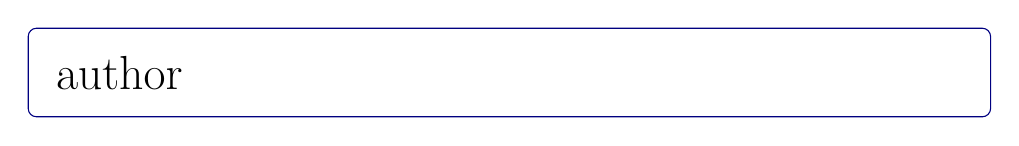
\begin{tikzpicture}
\node[rectangle,rounded corners=3pt,inner sep=10pt,draw=blue!50!black,text width= 0.95\textwidth] {\LARGE \@author};
\end{tikzpicture}
\end{minipage}
\bigskip\bigskip
}%
\makeatother

% custom section
\usepackage[explicit]{titlesec}
\newcommand*\sectionlabel{}
\titleformat{\section}
  {\gdef\sectionlabel{}
   \normalfont\sffamily\Large\bfseries\scshape}
  {\gdef\sectionlabel{\thesection\ }}{0pt}
  {
\noindent
\begin{tikzpicture}
\node[rectangle,rounded corners=3pt,inner sep=4pt,fill=blue!50!black,text width= 0.95\columnwidth] {\color{white}\sectionlabel#1};
\end{tikzpicture}
  }
\titlespacing*{\section}{0pt}{15pt}{10pt}


% custom footer
\usepackage{fancyhdr}
\makeatletter
%\pagestyle{fancy}
\fancyhead{}
%\fancyfoot[C]{\footnotesize \textcopyright\ \@date\ \ \@author}
\renewcommand{\headrulewidth}{0pt}
\renewcommand{\footrulewidth}{0pt}
\makeatother

\raggedbottom 
\usepackage{tikz-3dplot}
\begin{document}

%\maketitle

\begin{multicols*}{3}




\section*{Greek Characters}
\vspace{-0.35in}
\begin{tabular}{|L | L| L|} \hline
\mbox{Name} & \mbox{Symbol} & \mbox{Typical use(s)} \\ \hline
\mathrm{alpha} & \alpha  & \mbox{ angle, constant} \\
\mathrm{beta} & \beta  & \mbox{ angle, constant}  \\ 
\mathrm{gamma} & \gamma & \mbox{angle, constant} \\
\mathrm{delta} & \delta  & \mbox{ limit definition}\\
\mathrm{epsilon} & \epsilon  \mbox{ or } \varepsilon & \mbox{limit definition} \\
\mathrm{theta}  & \theta  \mbox{ or } \vartheta &\mbox{ angle}\\ 
\mathrm{pi} & \pi \mbox{ or } \uppi & \mbox{circular constant} \\
\mathrm{phi} & \phi \mbox{ or } \varphi  & \mbox{ angle, constant} \\

\hline
\end{tabular}

\vspace{-0.1in}

\section*{Named Sets}

\vspace{-0.35in}
\begin{tabular}{|L | L |} \hline 
\mathrm{empty\,\, set} & \varnothing \\ 
\mathrm{real\,\, numbers} & \mathbf{R} \\
\mathrm{ordered \, \, pairs }  & \mathbf{R}^2 \\
\mathrm{integers } & \mathbf{Z} \\
\mathrm{positive \,\,  integers } & \mathbf{Z}_{>0} \\ 
\mathrm{positive \,\, real \,\,  numbers} & \mathbf{R}_{>0} \\
\hline
\end{tabular}

\section*{Set Symbols}
\vspace{-0.35in}
%The \emph{union} is the members that belong to both sets; the \emph{intersection} are the members that belong to both sets.

\begin{tabular}{|L | L|} \hline
\mbox{Meaning}  & \mbox{Symbol} \\ \hline
\mathrm{is \,\, a \,\, member} & \in \\
\mathrm{subset}       & \subset \\
\mathrm{intersection} & \cap \\
\mathrm{union} & \cup  \\ 
\mathrm{set \,\,  minus}  & \setminus \\ \hline
\end{tabular}

%\vspace{0.1in}

%\noindent For sets \(A\) and \(B\), the statement \(A \subset B\) is true
%when every member of \(A\) is a member of \(B\).
\section*{Intervals}
\vspace{-0.35in}
\begin{minipage}[c]{0.333\textwidth}
For numbers \(a\) and \(b\), we define the intervals:
\begin{align*}
 (a,b) &= \left\{x \in \reals \ssep a < x < b \right\}  \\
  [a,b) &= \{x  \in \reals  \ssep a \leq  x < b \} \\
   (a,b] &= \{x  \in \reals \ssep a <  x \leq  b \} \\
    [a,b]  &= \{x  \in \reals \ssep a \leq  x \leq  b \} \\
 %   (-\infty, a) &= \{x \mid x < a \} \\
 %   (-\infty, a] &= \{x \mid x \leq  a \} \\
 % (a, \infty)  &= \{x \mid a < x  \} \\
 %  [a, \infty)  &= \{x \mid a \leq  x  \} \\
\end{align*}  
\end{minipage}
\vspace{-0.35in}

\section*{Logic Symbols}
\vspace{-0.35in}
%In mathematical logic, \(\ma{True or  True} \) is true.
\begin{tabular}{|L | L|} \hline 
\mbox{Meaning}  & \mbox{Symbol} \\ \hline 
\mathrm{negation} &  \lnot   \\
\mathrm{and} &  \land  \\
\mathrm{or} &  \lor  \\
\mathrm{implies} &  \implies  \\
\mathrm{equivalent} &  \equiv \\ 
\mbox{for all} & \forall \\
\mbox{there exists} & \exists \\ \hline
\end{tabular}


%To view a copy of this license, visit \url{https://creativecommons.org/publicdomain/zero/1.0 }
%\vspace{0.25in}
%\tiny
\noindent Revised \today. Barton Willis is the author of this work. This work is
licensed under Attribution 4.0 International (CC BY 4.0) \,  \qrcode[height=0.15in]{https://creativecommons.org/licenses/by/4.0/}. For the current version of
this document, visit \, \qrcode[height=0.15in]{https://github.com/barton-willis/Math-100-200-level} 

\end{multicols*}

\end{document}